\begin{figure}[H]
    \centering
    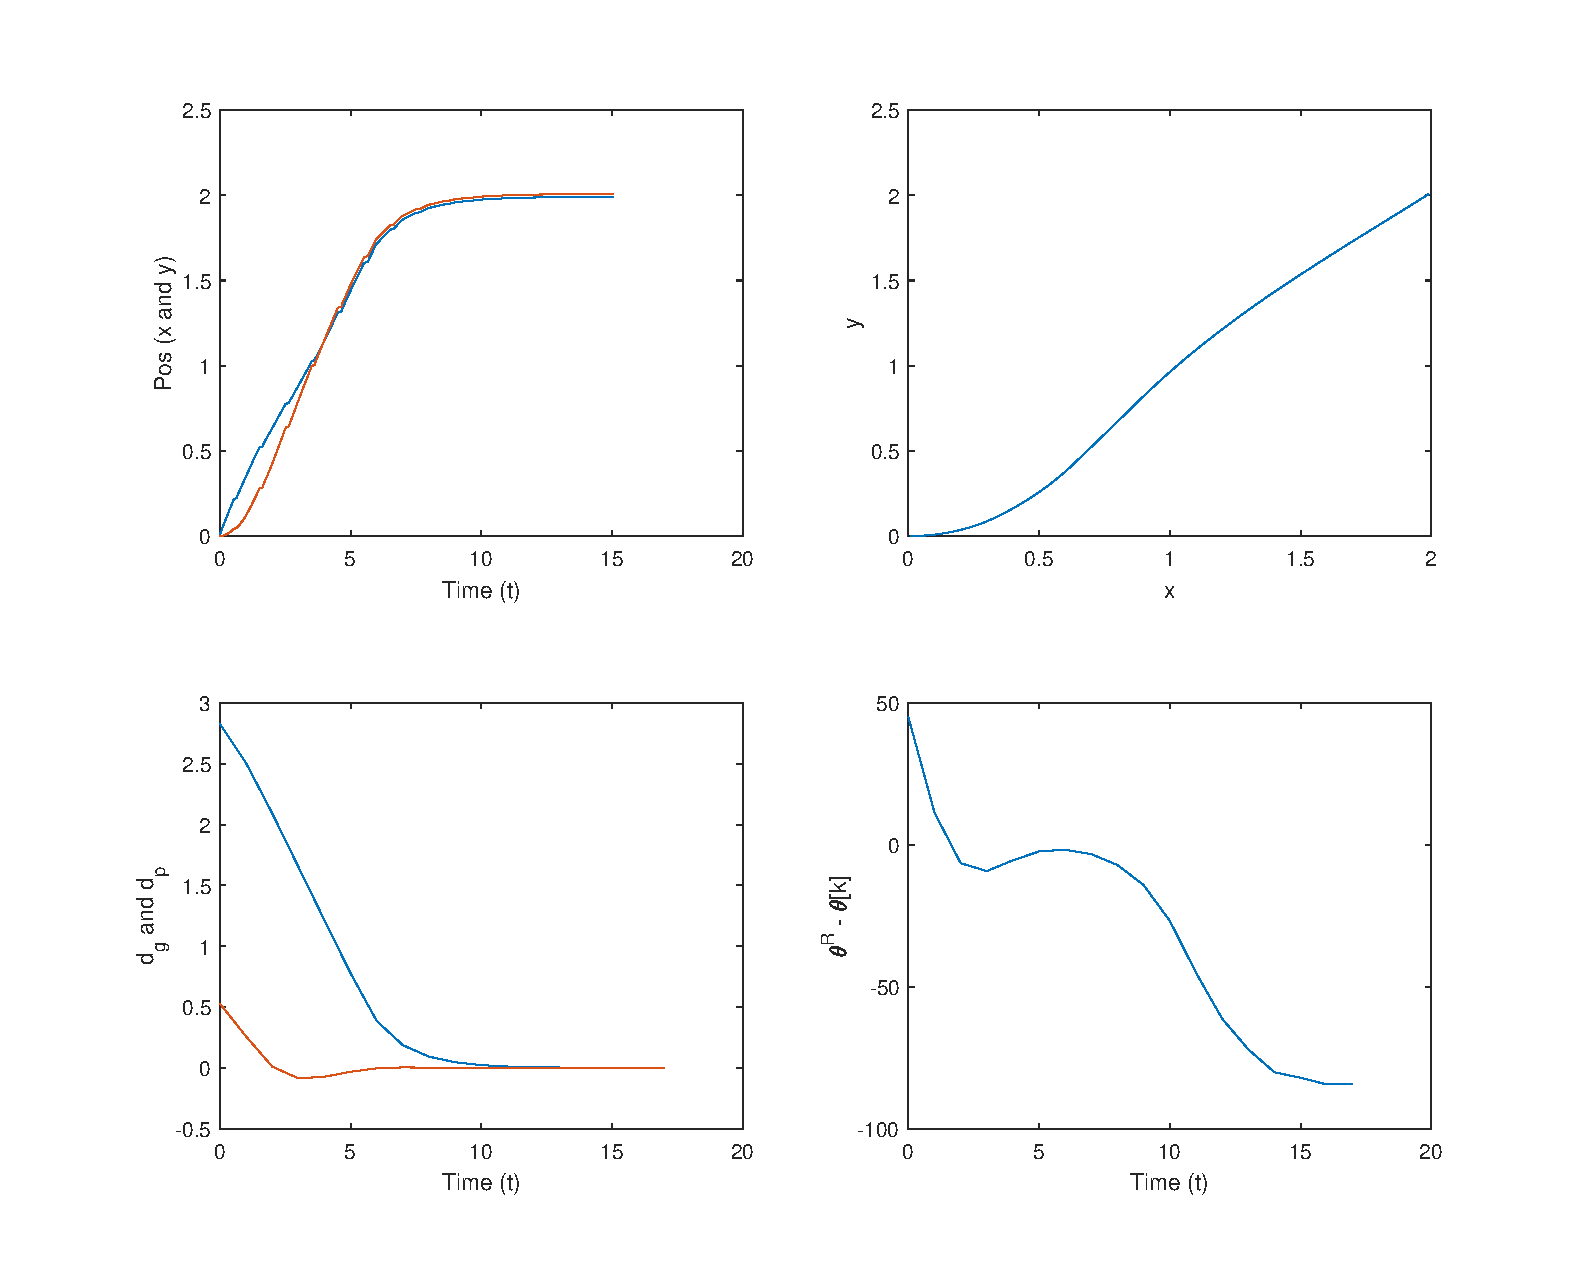
\includegraphics[width=\textwidth]{figs/perf-follow.eps}
    \caption{Simulation of the combined $d_g$ and $d_p$ controller going from $(0, 0)$ to $(2, 2)$ with $K_\omega = \frac{180}{R\pi}$, $K_\psi = \frac{180}{\pi} \frac{L}{Rp}$ and $p = 0.75$}\label{fig:perf-dg}
\end{figure}

As can be seen in \ref{fig:perf-dg}, the $d_g$ error evolve in an almost identical way to when the controller is used separately. However the $d_p$ error get a small overshoot compared to the separate case. This is likely from the virtual point getting pushed through the line by the velocity controller.